\documentclass[../dejiny-rodu-prusiku.tex]{subfiles}

\begin{document}

% str 23 @ 34
\section{Odnož Horní Bříza I větve Výrov}

Potomci Anny Prusíkové z Výrova, provdané Štěpánkové.

1805 - 1883

První dítě Vojtěcha Prusíka a Anny roz. Fenclové z Výrova byla Anna. Jak jsme již předtím uvedli, narodila se v době největší slávy Napoleonovy 4. ledna 1805 ve Výrově. Otec našel jí ženicha v rychtáři Jakubu Štěpánkovi z Horní Břízy č. 8, kde se odedávna říkalo u Kubíků. Po bitvě na Bílé Hoře bylo manětínskému pánu Kryštofu Karlu z Roupova, který právě ve stavov­ských bouřích zemřel, zkonfiskováno jmění. Koupila je Estera Mitrovská, rozená Lažanská, veliká katolička. Její manžel, Jiří Mitrovský z Nemyšle, přísný katolický pán, přitrhl hned s brannou mocí do Manětína, aby pro­vedl protireformaci. Kněz podobojí byl z Manětína od­straněn a povolán jesuita Jan Nerovius. Manětínští utrakvisté ve svém zpustošeném městě houževnatě vzdorovali. Shromáždili se na radnici, zavázali se přísahou, že neodstoupí od kališnictví, ale na přísnou pohrůžku Mitrovského se osm radních osob zavázalo písemně, že se stanou katolíky. Ostatní však po domluvě radního Štěpánka, který byl mlynářem na mlýně Růžkovském, odmítli přestoupiti.

Tento Štěpánek je předkem Jakuba Štěpánka, jehož si v XIX. století vzala za muže Anna Prusíková z Výrova. Pře­dek jeho, jako hlavní rebel, byl povolán na zámek, kde měl být ukován do železných pout. Odtud otevřeným oknem vyskočil a chtěl prchnout. Byl však poraněn a dopaden a v poutech poslán do Plzně. Když se to měšťané v Manětíně dověděli, chopili se zbraní a oblehli zámek. Vojsko narychlo povolané z Plzně, vzpouru však záhy potlačilo. V usedlosti potomka tohoto rebela žila tedy pak Anna. Vdala se sem 10. září 1822. Její muž Jakub narodil se v roce 1797, držel grunt do roku 1849 a zemřel 10. červen­ce 1869 v Horní Bříze. Na jejich gruntě bývala rychta. Anna zemřela 11. 3. 1883.

Anna s Jakubem měli šest dětí, které dospěly. Byla to nejdříve Marie, která se narodila 24. 6. 1824. Provdala se v roce 1843 do č. 2 ve Lhotce u Všerub na Plzeňsku za sedláka Václava Dobrého. Tam zemřela 20. 10. 1903.  Další byl Antonín Štěpánek naroz. 17. 11. 1831, zemřel 23. 3. 1841. Třetí dítě, Josef, stal se od roku 1849 dě­dicem gruntu. Byl z dvojčat, jeho bratr Vojtěch brzy zemřel. Narodil se 11. 3. 1828, zemřel 9. 1. 1902. Dcerka Anna narodila se 16. 9. 1834 a zemřela mladá 21. 2. 1845. Páté dítě, které dospělo, byla Barbora. Narodila se 3. 2. 1838, provdala se za Vojtěcha Kabáta v blízkém Ži­lově a zemřela tam 18. 1. 1910. Poslední, Antonín, druhý chlapec s tímto jménem, narodil se 28. 11. 1844. Zůstal po celý život starým mládencem a zemřel ve svém rodišti 20. 1. 1916.

% str 24 @ 35
Marie Dobrá, rozená Štěpánková, usazená ve Lhotce, byla podle vyprávění pamětníků, neobyčejně statečnou ženou. Nebyla jen dobrou selkou, ale nebála se ani chopit se v noci pušky a zahnati výstřely lupiče. Měla tři děti, které dospěly. Byl to Matěj nar. 18. 12. 1855. Zemřel svobodný ani ne dvacetiletý 10. 4. 1875. On byl předurčen jako dědic gruntu. Další Marie narodila se 24. 8. 1848 a provdala se opět ve Lhotce za Jana Dobrého, kde zemřela 21. 4. 1893. Druhý syn Václav byl narozen 1. 10. 1860 a byl dán na studie do Plzně. Když však jeho starší bratr Matěj tak brzy zemřel, vrátil se domů, ujal se gruntu a zemřel u dcery 19. 8. 1944 v Příšově.

Marie Dobrá, provdaná za Jana Dobrého v č. 3 ve Lhotce měla pět dětí. Byla to dobrá máma a hospodyně, ale svůj život skončila brzy. Zemřela po potratu ve svých 45 letech. Nejstarší syn byl Matěj nar. 31. 10. 1873, zemřel 13. 8. 1949 v Plzni. Matěj vystudoval lékařství a když v jeho době začínal u nás zvýšený zájem o dětskou lékařskou péči, usadil se s tímto zaměřením v Plzni a je považován za prvního odborného dětského lékaře v západních Čechách. Míval velikou klientelu ze všech kruhů obyvatelstva i z bývalé šlechty. Lékař Matěj Dobrý měl čtyři dcery. Nejstarší Sylva nar. 7. 2. 1903 provdaná nejdříve Fryčková. Podruhé si vzala Dr. Jiřího Havelku, ministra v Háchově vládě za protektorátu v nejtěžších dobách naší republiky. Její muž byl velký vlastenec a zatčen byl Němci spolu s předsedou vlády gen. Eliášem za heydrichiády. Dožil se sice osvobození a Sylva s ním, ale museli vytrpěti vel­ká příkoří. Museli se vystěhovat z Prahy do Hostomic pod Brdy. Z jejich manželství narodil se syn Jan 23. 3. 1943.

Druhou dcerou Matěje jest Zdeňka provd. Šperlová v Plzni, Škrétova 23. Narodila se 7. 2. 1908. Má dvě dcery, lékařku Zdeňku, provd. Klapálkovou, naroz. 15. 9. 1931 a Helenu, nar. 10. 2. 1944.

Třetí dcerou jest Milada, komerční ing., provd. za lékaře Dr. Semotána v Praze Bohnicích č. 138. Narodila se 10. 6. 1914. Děti nemá.

Čtvrtou je Květa, dosud svobodná, úřednice, bytem Praha - Strašnice, Na Hroudě 8. narodila se 19. 8. 1919.

Dalším dítětem Marie Dobré byla Anna. Narodila se 11. 11. 1882 a provdala se zase za sedláka Dobrého do Nevřeně. Zemřela v 81 letech 11. 3. 1963 u dcery v Radčicích u Plzně. Její syn Václav Dobrý nar. 17. 5. 1903, převzal pak hospo­dářství v Nevřeni č. 11. Má dceru Jiřinu, provdanou Jindrákovou nar. 5. 11. 1928. Ta má tři dcerky, Jiřinu nar. 25. 5. 1952, Miladu nar. 9. 1. 1954 a Soňu nar. 2. 8. 1963. Druhá dcera je Zdeňka, provd. Sedláčková, nar. 28. 6. 1930 bytem na stát­ním statku v Kunějovicích u Všerub. Má dva chlapce, Vladimíra nar. 8. 6. 1954 a Miroslava nar. 31. 12. 1956.

% str 25 @ 36
Bratr Václava z Nevřeně, je Ladislav Dobrý, naroz. 19. 7. 1911. Žije ve Stodě u Plzně, Na Jízdárně 429. Má syna Václava nar. 15. 12. 1937 a Annu. provd. Černou, v Mariánských Lázních - Úšovice, Polní 484-5b. Je narozena 14. 10. 1944 a má dcerku Kamilu nar. 19. 1. 1967. Sestra Václava a Ladislava, Anna, provdaná za učitele Randu. Je narozena 1. 3. 1909 a žila v Radčicích. Nyní bydlí v Plzni-Doubravce, ul. Družby 7. Má dceru Ja­roslavu, provd. Bezděkovou, naroz. 31. 8. 1933 v Plzni-Čechurově, Ke dráze 10. Má Pavla nar. 14. 10. 1956 a Janu nar. 27. 9. 1961. Syn Ladislav Randa nar. 20. 10. 1935 má zase již syna Ladislava nar. 18. 5. 1964. Syn Václav nar. 16. 12. 1943 a Bořek nar. 25. 6. 1946 jsou ještě svobodní.

Po své matce, Marii, předčasně zemřelé ve Lhotce, převzal grunt její syn Václav. Narodil se 18. 10. 1877 a zemřel tam 4. 2. 1928. Měl 4 děti. Jeho syn Václav nar. 3. 10. 1905 převzal po něm hospodářství, dnes je jako většina země­dělců členem JZD. Žije ve Lhotce č. 3. Jeho dcera Jarmila, provd. Pivoňková nar. 13. 9. 1933 má dvě děti Annu nar. 27. 7. 1957 a Luboše nar. 5. 2. 1959. Další dcerou Václava je Anna, provd. Kalousová bytem v Plzni-Slovanech, Mládežnická 29. Má dcerku Janu nar. 14. 5. 1961. Sama se narodila ve Lhot­ce 18. 3. 1937. Bratr Václava, Karel Dobrý, stal se právníkem, ale musil jako mnozí v době kultu osobnosti a růz­ných přehmatů, měniti často místo svého povolání, neúměr­ně ke svému vzdělání. Narodil se 19. 2. 1907. Bydlí v Českých Budějovicích, Komenského 65. Jeho syn Karel je lékařem v Plzni, Koperníkova 25, narozen 25. 10. 1938. Dcera Jitka, je narozena 22. 10.1945. Karel působí tč. v Karl. Varech. Syn Marie Dobré, Josef narodil se 17. 1. 1904. Byl úřední­kem v Hospodářském družstvu v Plzni a zemřel v Třemošné 27. 4. 1957. Měl syna Josefa nar. 29. 8. 1928, který žije v Plzni, Nám. J. Krautvurma 33. Má dvě děti: Evu nar. 16. 10. 1951 a Josefa 10. 6. 1958. Poslední byla dcera Anna nar. 28. 4. 1908. Měla za manžela Caltu, hajného v Horní Bříze. Její syn Milan, stal se les­níkem a bydlí ve Špindlerově Mlýně v Krkonoších č. 247. Narodil se 9. 7. 1927. Má synka Mirka nar. 12. 9. 1953. Dce­ra Zdeňka, provd. Ondráčková nar. 25. 8. 1929, má za muže letce. Bydlí v Praze na Smíchově, K vodojemu 210-11. Má dvojčata Pavla a Luboše nar. 20. 8. 1955.

Marie Dobrá ze Lhotky měla dalšího syna Emanuela. Narodil se 14. 1. 1885 a byl zaměstnán v železničních dílnách v Plzni. Zemřel poměrně brzy, 29. 5. 1940. Měl tři dcery a všechny učitelky. Jiřina provd. Kacerovská nar. 10. 4. 1914 a bydlí v Praze IV. Pankrác, I, Milevská 1088. Zdeňka, svobodná, nar. 28. 12. 1915 bydlí v Mariánských Lázních, Jiráskova 490, a Bohumila také svobodná nar. 6. 7. 1917 žije v Plzni, Božkovská 55. Po Emanuelu Dobrém není již žádných vnoučat.

% str 26 @ 37
Marie Dobrá měla ještě dceru, která dostala její Jméno. Narodila 15. 7. 1880 ve Lhotce a již v mládí měla tou­hu stati se jeptiškou. Skutečně také vstoupila do řádu Šedých sester a byla velmi obětavou sestrou v nemocnici. Když řádila španělská chřipka, nakazila se a zemřela 21. 9. 1916. Pod jménem Marie Libora najdete její hrob na Vyšehradě ve zvláštním oddělení řeholnic tohoto řádu.

Václav Dobrý nar. 1. 10. 1860 ve Lhotce č. 2 stal se dal­ším držitelem gruntu. Protože již okusil radosti města, když studoval v Plzni a musil se pak vrátit po časné smrti svého bratra Matěje domů, nikdy neměl velkou lásku k zemědělství. Jak vypravují pamětníci, nejraději měl lov a společnost. Nejstarším jeho dítětem byla Marie, nar. 13. 3. 1884. Je provdaná za pekaře Henžlíka v Kaznějově. Vzala si ho jako vdovce. Měla s ním dvě dcery. Starší Helena provd. Reinvartová v Kaznějově č. 90 je narozena 8. 4. 1915. Má tři děti: Alenu, která si po pro­vdání ponechala své jméno.  Je narozena 19. 6. 1940. Má synka Miroslava nar. 10. 11. 1963. Petr Reinvart je naro­zen 25. 9. 1949 a Pavel 1. 12. 1950. Druhá dcera Marie Henžlíkové je Zdeňka, provd. Hanzová v Kaznějove č. 304. Je narozena 14. 6. 1920. Má čtyři děti. Jaroslav nar. 9. 12. 1940 má již syna Radka nar. 12. 9. 1963. Zdeněk Hanza, nar. 27. 2. 1943 má syna Dušana nar. 10. 2. 1966. Jana, provd. Linhartová nar. 9. 11. 1944 má synka Jiřího nar. 10. 12. 1966, Irena Hanzová nar. 22. 4. 1949 je dosud vobodná. Alena Reinvartová má též dcerku Moniku, narozenou 13. 1. 1968.

Bratr Marie, Emanuel Dobrý narodil se ve Lhotce 3. 6. 1886. V sedmnácti letech onemocněl těžkým kloubovým revmatismem a mnoho let vytrpěl než jeho zesláblé tělo podlehlo. Zemřel ve svém rodišti 23. 2. 1927.

Václav Dobrý nar. 3. 2. 1889 ve Lhotce stal se učitelem. Působil na Roudnicku, v Bolevci u Plzně a v Ledcích. Žije nyní jako vdovec v Brníkově č. 108, pošta Ředhošť u Libochovic. Učitel Václav Dobrý je snad jediný, který zná dobře historii rodiny Dobrých a tedy život a osudy všech potomků Marie Dobré, roz. Štěpánkové z Horní Břizy. To byla jeho babička. Ze dvou synů, Miloslav naroz. 16. 8. 1922 skončil nešťastně svůj život 8. 11. 1936 - otrávil se. Druhý Václav, nar. 16. 8. 1922. Jeho dcera Jitka nar. 9. 5. 1952 žije s dědečkem v Brníkově. Nyní jako provdaná Větrová bydlí v Plzni, Máchova 15.

Jan Dobrý naroz. 24. 6. 1891 byl učitelem v Brozanech na Roudnicku, ale brzy zemřel na tyfus, svobodný. Dokončil svůj život ve svém rodišti 8. 8. 1913.

Další syn Václava Dobrého, Bohumil nar. 14. 1. 1894. Pocházel z dvojčat, ale jeho sestřička Bohumila, brzy zemřela. Převzal rodný grunt ve Lhotce č. 2, ale jeho manželství bylo bezdětné. Zemřel 2. 7. 1962.

% str 27 @ 38

Oldřich Dobrý narodil se 17. 3. 1897 ve Lhotce č. 2. Vyučil se pivovarnictví v Nekmíři a pracoval pak až do důchodu jako sladovnický dělník v Měšťanském pivovaře v Plzni. Bydlí v Záluží č. 118 u Plzně. Má dvě dcery. Zdeňka naroz. 8. 12. 1926 je provdaná Fol­ková v Senci u Zruče na Plzeňsku. Její muž je pokrevním členem rodu Prusíků. Mají dvě děti, Miloslava nar. 18. 11. 1949 a Jiřího nar. 28. 5. 1951. Další dcera Oldři­chova, Helena je provdaná Kubíková a žije s rodiči v Záluží. Je narozena 1. 12. 1929. Má dceru Zdeňku, nar. 23. 9. 1959.

Nejmladším dítětem Václava Dobrého ze Lhotky byla Helena. Narodila se 8. 4. 1903. Provdala se za rolníka a mlynáře Aloise Neužila v Příšově. Její dcera Marie je provdána Vodičková v Nýřanech. Narodila se 1. 5. 1930. Má dcerku Hanu nar. 26. 3. 1962. Syn Václav Neužil nar. 6. 1. 1934 žijící v Ledcích a je dosud otcem jednoho syna Václava nar. 5. 3. 1968. U Neužilů žil pak na výměnku starý hospodář Václav Dobrý ze Lhotky i se svou manželkou a tam také zemřel.

Učitel Václav Dobrý z Brníkova si svou babičku Marii Dobrou, roz. Štěpánkovou dobře pamatuje. Jako školačka docházela do školy ledecké, kam ve starší době byla Horní Bříza přiškolena. Zpívávala-li si píseň "Až já budu velká, bude ze mne selka" dočkala se toho, ale na růžích ustláno neměla, neboť práce bylo nad hlavu a zažila ještě robotu. Lhotka patřila k panství v Nekmíři. Pěstoval se len a doma se zpracovával na kolovrátku. Marie pracovala do pozdního věku jako výměnkářka a jak vzpomíná její vnuk, učitel Václav Dobrý, již ve 4 hodi­ny o žních budívala jeho otce a matku slovy: „Lidi vstá­vejte, už je čas, nebudete s prací hotovi!" A tak se robilo od slunka do slunka.

To je tedy krátké vyprávění o jednom z dětí Anny Prusíkové, provd. Štěpánkové a to o Marii Dobré, provdané ve Lhotce, na gruntě č. 2. Její potomci tam ještě ži­jí.

% str 28 @ 39
Synem Anny Prusíkové provdané Štěpánkové v Horní Bříze, byl Josef. Narodil se 11. 3. 1828 a když mu bylo 21 let převzal po svém otci Jakubovi rodný grunt č. 8. Bylo to v roce 1849, rok po zrušení roboty. Brzy se pak oženil s Marií Plevkovou z Kostelce nad Mží. Byl dobrým hospodářem a jejich statek patřil k největším ve vsi. Měl řadu dětí, o jejichž osudu si nyní povíme. Josef Štěpánek zemřel 9. 1. 1902.

Měl sedm dětí, které dospěly. Byly to: Kateřina provdaná Manclová v Horní Bříze. Narodila se 25. 11. 1852 a zemře­la 7. 3. 1938. Další dcerou byla Marie, provdaná Urbanová, rovněž v Horní Bříze. Narodila se v roce 1854, zemře­la 19. 5. 1894. Třetí, Anna také provdaná Manclová, ale v České Bříze, narodila se 30. 8. 1855, zemřela 23. 3. 1892. Syn Josef narodil se 6. 1. 1858 a zemřel 3. 5. 1936 v Horní Bříze. Antonín narodil se 7. 7. 1865, zemřel 20. 10. 1927 v Roudnici nad Labem. Jan, který pak převzal po otci grunt, narodil se 11. 5. 1868 a zemřel 27. 7. 1916. Posledním dítě­tem byla Josefa, která byla nervově chorá a zůstala svobodná. Narodila 28. 1. 1871 a zemřela ve svém rodišti po nešťastném životě 23. 5. 1918.

Kateřina Štěpánková narozená 25. 11. 1852 provdala se za sedláka Mancla v Horní Bříze a měla s ním pět dětí. Zemřela ve vysokém věku 86 let dne 7. 3. 1938. Její nejstarší dcera byla Anna. Narodila se 20. 6. 1873. Zemřela již 19. 11. 1913. Její dcera Josefa Sládková, jak byla provdaná její matka vzala si J. Ševčíka z Plas. Narodila se 1893 a zemře­la ještě rok před smrtí své matky v roce 1912. Ten rok se jí narodila dcerka Miloslava, která zemřela v roce 1932 svobodná na souchotiny /TBC/ jako její matka. Vojtěch Sládek narodil se 4. 3. 1897 a žije v Horní Bříze č. 19. Má čtyři dcery: Jarmila provd. Tylová v Ledcích č. 45 narodila se 19. 1. 1920. Má dcerku Jaroslavu nar. 24. 12. 1946. Další Marie je provdaná Hyčková narozená 29. 3. 1922 a ži­je v Plzni, Karlova 29. Má syna Jiřího naroz. 7. 8. 1949 a Magdalenu nar. 13. 7. 1953. Květuše je provdaná Frundlová v Trnové č. 22. Je narozená 8. 9. 1923. Její dvě děti jsou Pavel nar. 9. 2. 1946 a Květa naroz. 24. 7. 1948. Čtvrtá je Vojtěška, provdaná Patáková v Nýřanech č. 292. Narodila se 28. 5. 1929 a její dvojčata, Václav a Ludmila narodi­la se 7. 10. 1952.

Další dcerou Anny Sládkové byla Anežka. Narodila se 18. 3. 1895, provdala se za hostinského Kabáta na návsi v Horní Bříze č. 47 a zemřela 5. 8. 1953. Měla jediného syna, Jaroslava, který se narodil 4. 3. 1920. Vzal si za manžel­ku Miloslavu Kabátovou, která je také pokrevním členem našeho rodu, jako potomek dcery Marie sedláka Tomáše Prusíka z Horní Břízy. Jaroslav Kabát bydli v č. 90 a má tři chlapce. Václav nar. 7. 7. 1950, Jaroslav 31. 8. 1953 a Miloš nar. 2. 2. 1958. Druhým synem je Václav Sládek, nar. 30. 3. 1899. Bydli v Horní Bříze č. 324 a má Jediného syna Zdeňka, naroz. 19. 10. 1927 a ten má již zase dceru Zdeňku, nar. 3. 7. 1952. Václav Sládek zemřel 4. 6. 1966.

% str 29 @ 40
Pátým dítětem Anny Sládkové byla Marie. Narodila se 5. 6. 1901 a byla provdaná Brandtlíková v Trnové č. 161. Její syn Ladislav nar. 24. 5. 1923 zemřel již 7. 2. 1944. Dcera Božena nar. 22. 12. 1921 má dvě nemanželské děti. Její synek Ladislav nar. 4. 12. 1948 zemřel již když mu bylo 14 let 5. 6. 1962. Jedině její dcerka Helena nar. 3. 3. 1954 dělá jí radost ze života. Maminka Boženy Brandtlikové zemřela také poměrně mladá 14. 10. 1949. Opravdu některé rodiny mají tragické osudy. Božena Brantlíková zemřela 14. 2. 1969. Dcera Josefa narodila se 8. 4. 1876. Vzala si Václava Kroftu v Horní Bříze, kde zemřela 9. 3. 1954. Její syn, Václav narodil se 31. 7. 1895. Vzal si za manželku Annu, roz. Karezovou, která je také členem rodu Prusíků. Václav Krofta zemřel 23. 6. 1939. V tomto manželství se narodily čtyři děti. Nejstarší Dr. Vladimír Krofta, nar. 20. 1. 1920 a bydlí v Praze Dejvicích, Vilémovská 19. Působí na ministerstvu zdravotnictví. Má tři děti, Vladimíra nar. 10. 10. 1946, Martinu nar. 16. 12. 1948 a Tomá­še 13. 1. 1953. Dcera Jaroslava je provdaná Kokošková v Horní Bříze č. 125. Narodila se 31. 10. 1921 a má tři dě­ti. Vladimír nar. 12. 8. 1948, Jaroslava nar.15. 1. 1950, a Zdeňka nar. 11. 8. 1954. Zdeněk Krofta nar. 29. 7. 1925 je bezdětný a žije v Kupce u Teplic č. 358. Libuše, provdaná Šimicová v Horní Bříze č. 18 má tři dcerky. Václavka nar. 28. 9. 1950, Miloslava nar. 1. 7. 1952 a Libuše nar. 5. 9. 1953. Josefa Kroftová měla ještě dceru Barboru nar. 12. 11. 1902. Provdala se za úředníka Keramických závodů Šestáka, a má dceru Jiřinu, provdanou Šafaříkovou, narozenou 20. 6. 1923. Bydlí v Praze-Žižkově, Křížkovského č. 5.

Dcera Barbora narodila se 18. 10. 1882 (zemřela 18. 5. 1969.) a provdala se za hostinského Meistera v Horní Bříze č. 105. Má dva syny. Josef Meister narodil se 17. 2. 1913 a je technickým úřed­níkem. Bydlí v Praze Vršovicích, Tolstého 4. Jeho dvě děti jsou Zdeněk nar.11. 5. 1944 a Věra nar. 29. 11. 1948. Druhý syn Barbory, Adolf Meister narodil se 17. 6. 1921. Je úředníkem v Měšťanském pivovaru v Plzni. Bydlí s matkou v Horní Bříze. Jeho dcera Zdeňka narodila se 17. 5. 1947, synek Adolf narodil se 23. 5. 1951, ale 20. 8. 1964 se nešťastnou náhodou zastřelil z otcovy pušky. Jediný syn Kateřiny, Václav Mancl, narodil se v roce 1885. Byl svobodný. Padl ve světové válce na ruské frontě 1917. Posledním dítětem Kateřiny byla Marie. Narodila se 4. 7. 1887 a provdala se za učitele Smoláka v Horní Bříze, kde dodnes žije v č. 4. Má dva syny. Miroslav nar. 28. 9. 1920 je učitelem v Kadani. Bydlí tam v Chomutovské ulici č. 1219. Má čtyři děti: Miroslava narozená 19. 2. 1950, Pavel nar. 16. 1. 1952, Petr nar. 9. 8. 1953 a Marcela nar. 24. 7. 1957. Vlastimil Smolák narodil se 12. 2. 1922 a stal se knězem. Dnes působí na faře v Železné u Berouna č. 7. Zajímavé je, že kněz Smolák studoval a bydlil společně v semináři s jiným knězem Josefem Kouklem, který dnes působí v Kladrubech u Stříbra, ale tehdy oba nevěděli jistě, že mají v sobě společnou Prusíkovskou krev.

% str 30 @ 41
Druhou dcerou Josefa Štěpánka, držitele gruntu č. 8 v Horní Bříze byla Marie, provdaná Urbanová, také v Horní Bříze č. 22. Jak jsme již uvedli, zemřela mladá ve 40 letech 19. 5. 1894. Měla tři dcery. Dvě z nich také dlouho nežily. Anna narodila se 6. 5. 1883 a při kácení stromů v lese byla zabita. Stalo se to 16. 12. 1898. Na tomto místě ještě dnes připomíná neštěstí obrázek. Druhá její dcera Marie, byla provdaná Kryčová v Horní Bříze. Narodila se 11. 1. 1886 a zemřela v usedlosti, kde se narodila a žila, dne 23. 4. 1956. Měla dvě dcery: Marii provdanou Frundlovou, naroz. 11. 4. 1905, která zemřela 24. 7. 1925. Ta měla jediného syna Josefa naroz. 11. 11. 1923, který je usazen v Tlucné. Ten má dcerku Jaroslavu nar. v prosinci 1948. Druhá dcera Marie Kryčové je Anna naroz. 17. 2. 1907. Bydlí v Horní Bříze č. 81. Má tři děti. Hanu provd. Markovou nar. 21. 12. 1927. Ta bydlí rovněž v Horní Bříze č. 361. Má tři děti Hanu, nar. 23. 5. 1953, Václava nar. 29. 12. 1948 a Miroslava nar. 5. 8. 1954. Syn Josef Sopr naroz. 24. 1. 1933 bydlí s matkou. Má dvě děti, Jiřího nar. 5. 10. 1958 a Janu nar. 25. 7. 1961. Dcera Anna je provdaná Dobrá v Horní Bříze č. 236. Narodila se 12. 1. 1936 a má dvojčata Evu a Helenu, které se narodily 22. 12. 1956. Třetí dcerou Marie Urbanové byla Božena. Narodila se v roce 1889, byla pak provdaná Dlouhá v Kaznějově , ale tam zemřela bezdětná již v roce 1910.

Třetím dítětem Josefa Štěpánka byla Anna. Narodila se 3. 8. 1856 a provdala se jako Manclová do české Břízy. Tento rod je na gruntě usedlý již několik staletí. Když jí bylo teprve 36 let, zemřela tam 23. 3. 1892. Měla tři děti a z nich ještě dvě žijí. Její syn Václav Mancl na­rodil se 1. 3. 1880 a žije v gruntě svých předku na vý­měnku v České Bříze č. 1. Má tři děti. Syn Jaroslav na­rodil se 9. 2. 1913 a byl úředníkem Zeměměřického úřadu v Praze. Zemřel brzy, 14. 2. 1958. Jeho tři děti žijí v Plzni, Zbrojnícká č. 2. Marie narozená 11. 4. 1940 je provda­ná Pavelcová a má synka Jaroslava naroz. 9. 9. 1961. Její bratr je Jaroslav nar. 9. 10. 1945 a sestra Hana Manclová naroz. 17. 3. 1951. Druhým synem Václava Mancla je Rudolf. Narodil se 17. 4. 1914 a žije na rodném gruntě, kde dlou­ho odolával svodům kolektivního zemědělství. Má dvě děti, Václava naroz. 14. 10. 1947 a Jitku nar. 7. 2. 1950, která však v srpnu 1964 zemřela. Sestrou Jaroslava a Rudolfa byla Marie, která se narodila 13. 4. 1917, ale zemřela svobodná již 14. 8. 1935.

Druhým dítětem Anny Manclové byla Anna. Narodila se 11. 1. 1882, provdala se pak ke Klimešům do Horní Břízy. Tam zemřela 21. 11. 1953. Měla dvě dcery. Anna je provdaná Rajšlová nar. 13. 1. 1913 a žije v Horní Bříze č. 354. Má dce­ru Alenu, provd. Dienstbierovou nar. 23. 7. 1937 a ta má již chlapce Aloise nar. 16. 3. 1961. Druhou dcerou Anny Klime­šové je Marie. Narodila se 1. 1. 1917, provdala se k Do­lejšům v Horní Bříze č. 27. Má dvě děti: Václava nar. 20. 6. 1943 a Helenu nar. 2. 11 .1946.

% str 31 @ 42
Třetím dítětem Anny Menclové byla Marie. Narodila se 4. 9. 1886 a je provdaná jako Suchá ve Zruči č. 15  u Plzně. V rodě Suchých je majetkem grunt od roku 1756. Má jediného syna Jaroslava, naroz. 26. 8. 1912. Vystudoval gymnasium v Plzni, ale po studiích vrátil se domů a je tam stále ještě soukromým sedlákem. Má čtyři děti. Anna provd. Honomichlová je narozena 26. 3. 1945 a má již dcerku Hanu roz. 29. 11. 1966. Další dcerou Jaroslava Suchého je Helena, naroz. 5. 9. 1948, Marie nar. 3. 11. 1951 a Jitka nar. 24. 7. 1955.

Čtvrtým dítětem Josefa Štěpánka byl Josef. Narodil se 6. 1. 1858. Byl dán na studie do Plzně, poněvadž bylo určeno, že grunt dostane jeho mladší bratr Jan. Stal se později berním úředníkem, ale vysedávání v kanceláři se mu nezalíbilo. Vrátil se poměrné brzy opět do svého rodiště a usadil se tam v č. 2 a sedlačil. Měl čtyři dě­ti. Jeho dcera Barbora naroz. 10. 11. 1885 je provdaná Honomichlová a žije v Plzni, Slovanská tř. 67. Děti neměla. Druhým dítětem jeho byla Anežka. Narodila se 31. 10. 1893. Provdala se později za vdovce Václava Šíra, úřed­níka Kaolinky, který z prvního svého manželství má syna, který působí jako profesor v Chocni. Anežka sama vlastní děti neměla. Žije v Horní Bříze č. 219. Josef Štěpánek měl dále dva syny. Václav narodil se 8. 1. 1896 a hospodařil pak jako jeho otec v čísle 2. Zemřel 16. 2. 1962. Jeho děti jsou Václav naroz. 21. 2. 1922 a je dosud svobodný. Dlouho byl předsedou místního JZD. Sestra jeho Marie, provd. Zíková narodila se 19. 6. 1924 a žije v Dolanech u Třemošné. Má dvě děti, Václava nar. 18. 5. 1950 a Evu naroz. 2. 8. 1957. Druhým synem je Josef Štěpánek, nar. 25. 3. 1898. Je dělníkem v Keramických závodech a bydlí v domku č. 219 jako jeho sestra Eliška. Má tři děti. Zdeněk nar. 22. 3. 1941 bydlí v Třemošné č. 322. Má dvoj­čata dcerky Janu a Zdenku nar. 23. 1. 1964. Marta je provdaná Sýkorová v Senci u Plzně. Narodila se 28. 8. 1943 a má synka Miloslava nar. 1. 12. 1963. Konečně je Pavel Ště­pánek nar. 9. 6. 1947.

Pátým dítětem Josefa Štěpánka byl Antonín. Narodil se 7. 7. 1865. Také on šel na studie. V roce 1885 absolvoval Hospodářskou akademii v Táboře a pak ještě Lihovarnickou školu v Praze. Stal se hospodářským správcem a působil na mnoha velkostatcích a také dlouho v pivovaře v Praze-Bráníku. Nejdéle byl v Mlázovech u Kolince, ale také na velkostatku hraběte Harracha v Sadové na Kralovéhradecku, v Žinkovech u Plzně a jinde. V pozdním věku se oženil a usadil na Roudnicku, kde také zemřel 20. 10. 1927. Měl jediného syna Jiřího, který se narodil 1. 1. 1916. Je elektrotechnikem a žije ve Straškově č. 127 na Podřipsku. Má dvě dcery. Anna provd. Nováková nar. 22. 6. 1946, jejíž trvalé bydliště je Praha Žižkov, Bořivojova 90. Má syna Jiřího, nar. 30. 11. 1967. Její sestra Jitka, nar. 23. 11. 1947 je provdaná Králová v Černuci u Velvar.

% str 32 @ 43
Šestým dítětem Josefa Štěpánka byl Jan, nar. 11. 5. 1868. Převzal snad nejhezčí grunt v Horní Bříze, ale hospodaření nebylo zvlášť šťastné. Měl osm děti. Nejstarší byla Anna provd. za úředníka Kabáta v Otrokovicích u Zlí­na. Narodila se 13. 11. 1897. Zemřela na Moravě 25. 2. 1958. Měla dvě dcery. Starší je Anna nar. 28. 6. 1920. Je provdána za lékaře Dr. Jaska a v nedávných pohnutých dobách, zavál ji osud až do Austrálie. Žili tam již na různých místech jako ve státě Victoria, také v hlavním městě Cambeře a nyní v Melbourne. Jejich dcerka Marie naro­dila se v lednu 1964 a syn Michal 21. 11. 1964. Druhá dce­ra je Vlasta, provdána Sokolová a bydlí v Otrokovicích ul. Ivana Olbrachta č. 1193. Narodila se 11. 11. 1921. Má dvě děti, Alenu nar. 21. 3. 1942 provdanou Kedrovou, bytem v Otrokovicích č. 599. Ta má dva synky, Petra nar. 29. 6. 1963 a Jiřího nar. 9. 5. 1965. Milan Sokola, nar. 28. 4. 1944 má syna Bronislava nar. 19. 6. 1966. Po Janovi stal se držitelem gruntu Václav Štěpánek. Narodil se 3. 12. 1898. Když se ujímal hospodářství, bylo již velmi zadlužené. Chtěl celý grunty mající asi 30 ha udržet a vypůjčil si peníze na velký úrok. Přišla neúroda, nemoce a vše šlo s kopce. Statek byl prodán v draž­bě 20. 5. 1933. Václav se svou rodinou byl vystěhován na náves ke kapličce a začal pracovat v lese. Václav zemřel 21. 3. 1958 v Žilově, kde se nakonec postižená rodina usa­dila. Byl tedy Václav Štěpánek posledním hospodářem v č. 8 v Horní Bříze, kam se více než před 110 lety přivdala z Výrova Anna Prusíková. Děti Václava Štěpánka jsou: Václav nar. 7. 2. 1927, který dnes místo sedlačiny je za­městnán u Stavebních závodů v Plzni a možná, že je mu tam lépe. Bydlí v Plzni, Dukelská ul.12. Má dvě děti Hanu,  nar. 9. 3. 1958 a Václava nar. 26. 6. 1960.

Dcera Marie je provdaná Weberová a bydlí v Žilově v č. 9. Narodila 8. 12. 1930 a po svízelném mládí se jí opět dobře daří. Má dvě dcerky. Alenu nar. 1. 6. 1956 a Irenu nar. 21. 8. 1961.

Dalším dítětem Jana Štěpánka byla Marie. Narodila se 7. 12. 1900. Žije jako provdaná Marková v Záluží č. 29 u Plzně. Její dcera, Jaroslava nar. 13. 1. 1924 je provdaná Bláhová, a bydlí v Plzni, U tržiště 1. Druhá Olga, narodila se 2. 10. 1927, je provdaná Polcarová a žije s matkou v Třemošné. Syn František Marek, narodil se 15. 7. 1930 a když mu bylo 25 let skončil tragicky svůj život. Oběsil se 13. 2. 1955. Zanechal po sobě synka Jaroslava nar. 27. 4. 1949. Dcera Růžena nar. 22. 2. 1903 provdala se za úředníka Vysko­čila a mají vilku v Plzni-Slovanech, Květná č. 37. Zůsta­la bezdětná. Její sestra Božena narodila se 13. 10. 1904 a  provdala se za učitele Honomichla. Žije v Třemošné č. 98. Má jedinou dceru Boženu, provdanou Knákalovou. Narodila se 14. 5. 1925 a je profesorkou. Bydlí v Plzni, ul. Víta Nejedlého č. 18. Má syna Petra nar. 1. 8. 1955. Syn Jaroslav nar. 12. 6. 1906 zůstal svobodný. Pracuje v Keramických závodech v Třemošné a tam bydlí u své sestry Boženy. Jeho bratr Josef nar. 2. 2. 1909 je řídícím učitelem v Liticích nad Orlicí a je bezdětný. Jeho bratr Jan nar. 28. 2. 1912 je odborným učitelem v Oseku u Duchcova, Tyršova ul. 421. Má synka Kamila, nar. 8. 4. 1948.

% str 33 @ 44
Barbora byla druhou dcerou Anny Prusíková provdané Štěpánkové, která dospěla. Narodila se v Horní Bří­ze č. 8, 3. 2. 1838 ještě v době roboty. Provdala se do statku, kde se říkalo U Kardátů, do Žilová. Její muž byl sedlák, V. Kabát. Usedlost č. 2 je na návsi a patří mezi nejvýstavnější v obci. Na Barboru Kabátovou, roz. Štěpánkovou vzpomínala dlouho její vnou­čata jako na předobrou a štědrou babičku. Měla čtyři děti, které dospěly. Nejstarší byl Matěj Kabát, nar. 21. 2. 1862, který pak dále hospodařil na rodném statku. Zemřel 6. 11. 1914. Druhým dítětem byl Jan, nar. 25. 6. 1868. Byl inspektorem čsl. drah a zemřel v Plzni 28. 4. 1944. Dcera Marie narodila se 23. 1. 1871 a provdala se ke Švíglerům do Lhotky. Tam zemřela 14. 9. 1938. Nejmladší byla Anna, nar. 22. 12. 1877. Provdala se za Josefa Ebrle do dvora "U Kolečků“ v Třemošné. Zemřela tam 28. 11. 1957. Barbora Kabátová zemřela v 72 letech 18. 1. 1910 v Žilově.

Nejstarší syn Barbory Kabátové, Matěj nar. 21. 2. 1862, převzal po rodičích grunt v Žilově č. 2 a z jeho manželství narodilo se šest dětí. Nejstarší Vojtěch, nar. 5. 10. 1886 pracoval doma na statku, zůstal svo­bodný, ale jeho život skončil nešťastně. Oběsil se doma v Žilové, 28. 3. 1958. Druhým dítětem je Marie, provdaná Čechová, bytem v Žilově č. 21. Narodila se 25. 3. 1888 a má dva syny. Starší Ladislav Čech zůstal na statku. Narodil se 21. 3. 1915 a má děti: Marii nar. 26. 1. 1947, Ladislava nar. 2. 6. 1948, Miladu nar. 25. 8. 1951, Annu nar. 19. 4. 1954 a Helenu nar. 18. 3. 1961. Jeho bratr Karel nar. 7. 2. 1917 byl důstojníkem, ale nyní pracuje v jiném oboru. Bydlí v Praze — Žižkově, Sudoměřská 5. Má dceru Olgu, nar. 17. 12. 1946. Třetí je dcera Helena nar. 17. 4. 1897 a vzala si sedláka J. Dolejše z Hubenova u Plas. Tato dcera dostala rodný grunt. Má dva syny.

Josef nar. 18. 4. 1933 bydli v Žilově č. 23. Má jedno dítě: Josefa nar. 16. 7. 1958. Bratr jeho Václav Dolejš narodil se 19. 4. 1931 a bydli s rodiči. Má dvě dě­ti, Václava naroz. 8. 1. 1956 a Drahuši nar. 11. 12. 1958. Dcera Božena naroz. 29. 1. 1896 provdala se za soustružníka Hořejše do Křimic u Plzně. Má dvě děti. Dcera Svatava narodila se 1. 12. 1936 a je provdaná Kučerová v Plzni-Škvrňanech, U dráhy 7. Má dcerku Svatavu, nar. 20. 3. 1959. Bratr její Vratislav Hořejš nar. 25. 8. 1941 je svobodný.
Barbora, která dostala jméno po své bábě, roz. Štěpánkové narodila se 31. 3. 1894. Provdala se za hostinského v Nekmíři č. 9. Její syn Jaroslav Hyrát narodil se 8. 4. 1926 a bydlí také v Nekmíři. Pracuje v Plzni ve Škodovce. Má dva chlapce, Jaroslava nar. 18. 4. 1957 a Jana narozeného 13. 3. 1958. Bratr Jaroslavův je Miloslav a narodil se v Nekmíři 18. 9. 1928. Je inženýrem-agronomem.

Další dcera Matěje Kabáta byla Anna. Narodila se 21. 6. 1899 a poprvé byla provdána Týmrová a podruhé Mošnová. Bydlí v Plzni-Koterově, Na Hradčanech 100. Její dcera Jindřiška Mošnová nar. 1 .4. 1940 je dosud svobodná.

% str 34 @ 45
Třináct let před smrtí svého otce Matěje Kabáta, narodil se pak ještě Václav 11. 9. 1901. Zůstal svobodný, pracuje v zemědělství a bydlí u své sestry Heleny Dolejšové, v Žilově č. 2.

Druhým synem Barbory Kabátové byl Jan nar. 25. 6. 1868 v Žilově. Původně chtěl studovat lékařství, ale brzy toho zanechal a vstoupil do služeb čsl. drah. Dlouho působil ve Zlivi u Č. Budějovic, později byl na ředitelství drah v Plzni, kde zemřel 28. 4. 1944. Byl miláčkem své matky. Z jeho manželství narodili se tři synové a jedna dcera. František nar. 28. 11. 1896 byl elektromechanikem, usadil se v Brně. Dne 16. 10. 1942 narodil se mu syn Jan, který je dosud svobodný. František Kabát zahynul při náletu na Brno za druhé světové války 12. 4. 1945. Dru­hý syn Jan narodil se 2. 2. 1902. Byl úředníkem v Plzni, ale známé poměry po druhé světové válce, kdy často politika znamenala více než pracovní schopnost, donutily ho ke změně zaměstnání. Jan Kabát zemřel 14. 12. 1967 v Plzni raněn mrtvicí. Jeho syn Jan narodil se 15. 8. 1937 a bydlí v Plzni, U Radbuzy č. 18. Má syna Jana nar. 9. 10. 1961 a dceru Zdenku, nar. 31. 10. 1964. Jeho dcera Ludmila je provdaná Cibulková v Plzni. Narodila se 13. 4. 1942 a bydlí v Plzni - Bolevci, Čechova 71a. Má dcerku Markétu nar. 20. 3. 1965. Dcera Ludmila narodila se 9. 11. 1903 ve Zlivi jako ostat­ní děti a stala se magistrou farmacie. Byla provdaná Klí­mová, ale brzy ovdověla. Je bezdětná. Bydlí v Praze 7, Veletržní 15. Čtvrtým dítětem Jana Kabáta je Ladislav nar. 7. 12. 1904. Bydlí v Plzni, Lochotínská 57. Má tři děti. Dcera Jiřina, provdaná Veselá narodila se 22. 7. 1929. Bydlí v Litvíno­vě, Žižkova 658/2. a má synka Václava nar. 7. 3. 1948. Syn Stanislav Kabát nar. 23. 10. 1936 bydlí s otcem v Plzni, je ženatý a má dva synky. Stanislava nar. 2. 7. 1955 a Ji­řího, nar. 7. 12. 1956. Dcera Anna narodila se 21. 7. 1931. Byla provdaná Červencová, ale tragicky zahynula 31. 7. 1961. Skutečně, rodina Jana Kabáta ze Žilova byla často pronásledována neštěstím jak někdy se v živote stává.

Nejstarší dcerou Barbory Kabátové ze Žilová byla Marie. Narodila se tam 23. 1. 1871. Provdala se v r. 1899 za Václava Švíglera, sedláka ve Lhotce č. 1. Příbuzenstvo se stra­ny matky tam již měla a to potomky její tety Marie Dobré. Ta, když se tam Marie provdala, ještě žila a jistě byla dobrou rádkyní své neteře. Marie Švíglerová zemřela ve Lhotce těsně před zřízením protektorátu, kdy hranice s říší byly vedeny téměř za humny obce. Zemřela 14. 9. 1938. Měla šest dětí. Nejstarší byla Anežka. Narodila se 8. 6. 1894 ve Lhotce a provdala se za sedláka Vojtěcha Beránka do Vladměřic č. 5 u Manětína. Zemřela tam 29. 12. 1956. Zanechala po sobě ne­obyčejně četné potomstvo. Měla osm dětí. Nejstarší Vojtěch Beránek narodil se 29. 1. 920 a dnes žije v rodišti. Má

% str 35 @ 46
dvě děti, Václava nar. 22. 6. 1946 a Jarušku, nar. 31. 12. 1954. Marie nar. 3. 7. 1922 je provdaná Wollrábová v Plasích č. 53. Má četnou rodinu, tři dcery a dva syny. Dcera Marie je provdaná Soutnerová a žije také v Plasích č. 74. Narodila se 17. 2. 1941. Syn Josef je narozen 24. 10. 1960 a František nar. 7. 9. 1962. František Wollráb narodil se 29. 4. 1942, Růžena nar. 30. 5. 1947, Hanna 14. 12. 1951 a Vojtěch Wollráb 2. 12. 1955. Dalším dítětem Anežky je Helena. Je narozena 13. 8. 1924 a žije dnes, provdaná Bláhová v Manětině č. 63. Má dva syny a dceru. Jaroslav je narozen 22. 8. 1949, Zdeněk 8. 10. 1951 a Helena Bláhová 29. 9. 1958.

Václav Beránek narodil se 10. 1. 1928 a žije ve Vladměřicích. Ještě je svobodný. Jeho bratr František pochá­zí z dvojčat. Narodil se 29. 8. 1930 a žije dnes v Manětíně č. 1. Má synka Jiřího nar. 6. 4. 1958 a dceru Lud­milu nar. 16. 8. 1959. Jeho dvojče, sestra Anna je provdaná Pokorná a žije v Kolešově u Žlutíc. Má dceru Alenu nar. 18. 6. 1955 a dceru Jaroslavu nar. 7. 1. 1954. Další dcera Anežka, nar. 16. 11. 1932. Je provdaná Šedivá, a žije dnes v Krásném Údolí č. 68 u Toužimi. Má dvě dcerky, Miluši nar. 16. 12. 1955 a Hanu nar. 2. 9. 1958. Posledním dítětem Anežky Beránkové je Zdeňka. Narodila se 8. 1. 1938. Žije ve svém rodišti, kde se těší s nemanželskou dcerkou Bohuslavou nar. 11. 6. 1957.

Druhým dítětem Marie Švíglerové je Václav, nar. 17. 5. 1900. Převzal po rodičích statek ve Lhotce č. 1, který je dnes začleněn do JZD. Má dvě děti, Milada nar. 12. 1. 1938 je provdaná Čečilová a žije v Nevřeni č. 46. Má synka Milana nar. 16. 10. 1962. Její bratr Václav Švígler nar. 6. 2. 1939 zůstal ve Lhotce. Má dvě děti, Lenku nar. 1. 3. 1964 a Václava nar. 23. 6. 1965.

Třetí byla dcera Marie. Narodila se ve Lhotce 24. 6. 1903 a provdala se za rolníka Nového v Horní Bělé č. 18. Má dvě dcery. Miloslava nar. 19. 1. 1929 je provdaná Dobrá a má dvě děti; Miloslavu nar. 18. 8. 1953 a Oldřicha nar. 27. 2. 1957. Její sestra Marie nar. 21. 3. 1932 je provdaná Janouškovcová a má dvě dcery. Helenu nar. 7. 1. 1956 a Marii nar. 27. 12. 1957.

Další dcera byla Barbora. Narodila se 13. 5. 1908. Nejdříve byla provdaná Frundlová a z tohoto manželství má dvě dcery. Libuše je narozena 26. 5. 1933 a je provdaná Loukotová v Ledcích. Má dcerku Annu nar. 4. 6. 1959. Druhá dcera Anna je ještě svobodná. Narodila se 27. 10. 1935. Zemřela 10. 10. 1951. Barbora provdala se pak znovu jako Janouškovcová a žije v Trnové. Z tohoto druhého manželství má syna Václava nar. 10. 2. 1949.

Syn Josef Švígler nar. 27. 2. 1913 zůstal svobodný a pracuje v Plzni. Bydlí tam na Husově nám. č. 4. Posledním dítětem Marie Švíglerové ze Lhotky je Anna. Narodila se 28. 10. 1915. Provdala se do Plzně, za úřední­ka Škodovky. Bydlí v Plzni, Dobrovského ul. č. 7. Má dva syny: Jiřího Klímu, nar. 5. 11. 1940 a Jana nar. 2. 2. 1947.

% str 36 @ 47
Nejmladším dítětem Barbory Kabátové, roz. Štěpánkové, byla dcera Anna. Narodila se 22. 12. 1877. Provdala se v r. 1902 do Třemošné za rolníka Josefa Ebrle. Zemřela tam 28. 11. 1957. Měla šest dětí. Nejstarší byl Josef Ebrle. Narodil se 29. 6. 1904 a žije ve svém hospodářství v Třemošné č. 84 jako člen JZD. Má tři děti. Nejstarší Jindra narodila se 26. 7. 1929 a je provdaná Honomichlová v Tře­mošné. Má dva syny Stanislava nar. 1. 7. 1951 a Jindřicha, nar. 19. 5. 1959. Druhou dcerou je Miroslava provdaná Pašková, rovněž v Třemošné. Narodila se 25. 1. 1932 a má dvě děti. Otto nar. 9. 3. 1957 a dcera Miroslava nar. 27. 6. 1962. Druhé dítě Anny Ebrlové je Anna nar. 8. 7. 1906, provdaná za obchodníka Pospíšila v Plzni. Bydlí tam v Tylově ulici č. 47. Má syna Jiřího nar. 18. 4. 1941, který má již dcerku Ivettu nar. 26. 1. 1965.

Třetí byl syn Rudolf, nar. 4. 4. 1909. Je bezdětný a půso­bí jako náčelník stanice ČSD v Berouně. Dalším synem je Václav Ebrle, nar. 2. 7. 1912 v Třemošné. Usadil se v Záluží č. 141. Je krajským dispečerem Západočeských elektráren. Má dva syny, Václava nar. 26. 12. 1943 a Vladimíra nar. 3. 10. 1950.

Marie narodila se 3. 6. 1914. Provdala se za rolníka Peška, který je nyní členem JZD v Záluží. Bydlí v č. 22. Má dce­ru Janu, nar. 21. 10. 1945 a syna Jana nar. 21. 9. 1952. Nejmladším dítětem Anny Ebrlové z Třemošné byla Milosla­va. Narodila se 14. 4. 1918. Provdala se za plukovníka Bayerle, rodáka ze Žilova, který si však změnil jméno na Borský. Bydlí v Praze 6 Na větrníku č. 1487. Miloslava Borská má tři děti. Nejstarší Pavel nar. 8. 5. 1942 je inženýrem. Dcera Jana provd. Zábranská, nar. 19. 1.1945. Má dceru Tamaru nar. 19. 4. 1964 a Ivanu nar. 4. 4. 1966. Třetí dcera Miloslava Borská narodila se 6. 4. 1946 a je učitelkou.

Tím končíme stručné vyprávění o živých a mrtvých potomcích dcery rychtáře Vojtěcha Prusíka z Výrova, Anny provdané Štěpánkové v Horní Bříze před více než 165 lety. Snad bude zajímavé když uvedeme počet jejích potomku až k dnešku. Je to úctyhodné číslo 37o lidí, z toho 58 mrtvých. Samo­zřejmě, obrázek tento mění se velmi rychle, tak jak je náš život proměnlivý, ale ke dni, kdy končíme toto vyprávění, je snad počet potomků pozoruhodný.

% str 36+1 @ 48
\begin{figure}
\centering
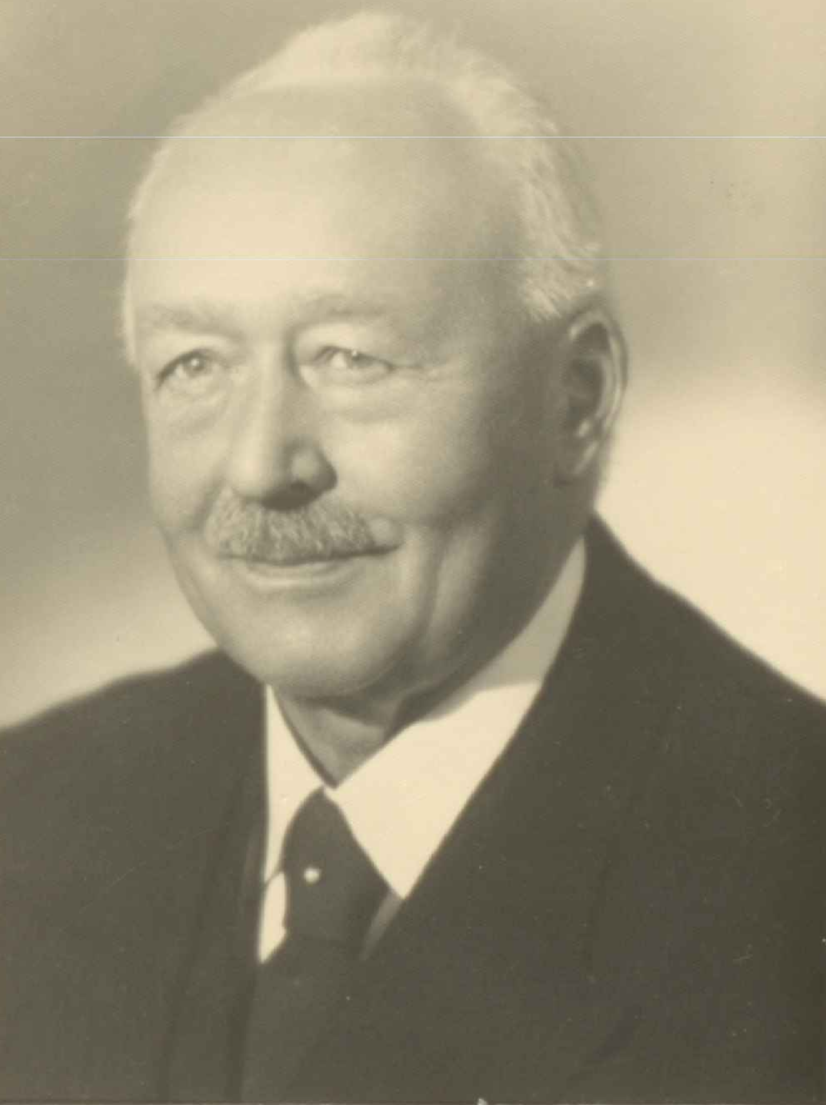
\includegraphics[width=\textwidth, height=\textheight, keepaspectratio]{048-a-matej_dobry}
\caption{MUDr. Matěj Dobrý, první dětský lékař v západních Čechách (1873 – 1949);
Potomek Anny Štěpánkové z Horní Břízy, rozené (1805) Prusíkové ve Výrově}
\label{fig:048-a-matej_dobry}
\end{figure}

\begin{figure}
\centering
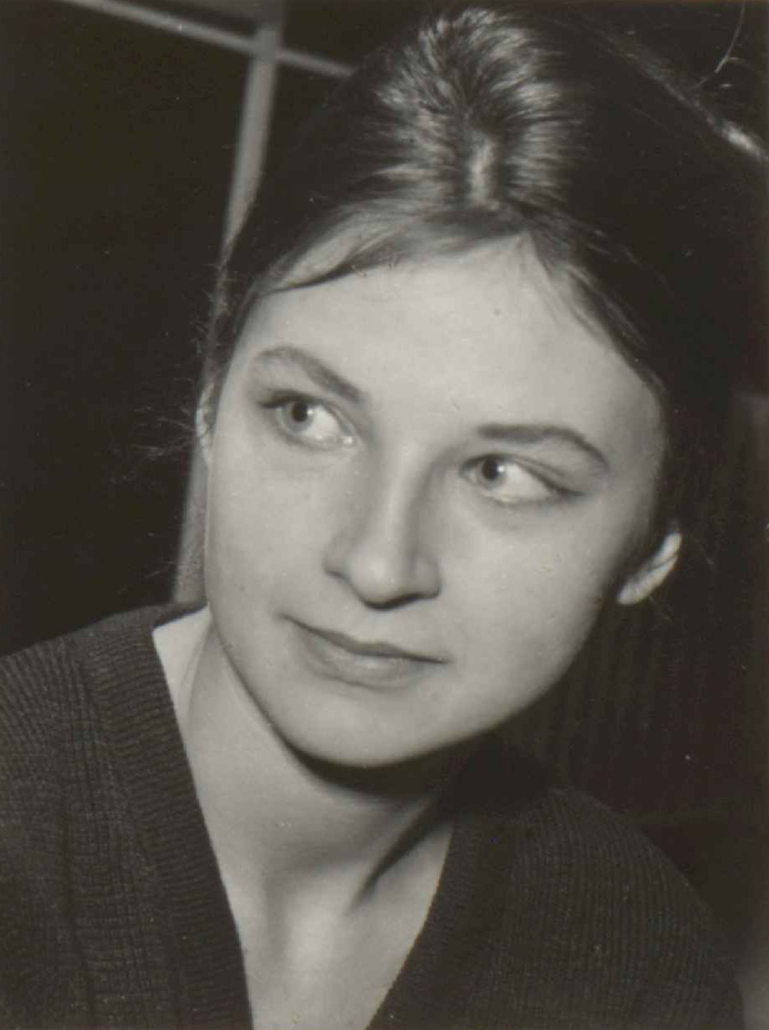
\includegraphics[width=\textwidth, height=\textheight, keepaspectratio]{048-b-jindra_karasova}
\caption{Jindra Karasová, operní pěvkyně, potomek Rosálie Karasové z Horní Břízy, rozené Prusíkové ve Výrově}
\label{fig:048-b-jindra_karasova}
\end{figure}


\end{document}
